%\documentclass[a4paper,12pt,oneside,draft]{article}
\documentclass[a4paper,12pt,oneside]{article}

% In the original writelatex tamplate
\usepackage[english]{babel}
\usepackage[utf8]{inputenc}
\usepackage{amsmath}
\usepackage{graphicx}
\usepackage[colorinlistoftodos]{todonotes}

% By LoCigno
\usepackage{times}
\usepackage{graphicx}
\usepackage{subfigure}
\usepackage{csvsimple}
\usepackage{color}
\usepackage{url}
\usepackage{hyperref} 
\usepackage{cleveref}

% By Davide
\usepackage{comment}
\usepackage{booktabs}
\usepackage{color}

%Variables macros
\newcommand{\DefineVar}[2]{%
  \expandafter\newcommand\csname var-#1\endcsname{#2}%
} 
\newcommand{\var}[1]{\csname var-#1\endcsname}

\usepackage{courier}
\newcommand{\mono}[1]{\texttt{#1}}
%\newcommand{\mono}[1]{\texttt{\textbf{#1}}}

\title{Identification procedure for Lego Mindstorm motor}

\author{Diego Verona, Aliaksandr Siarohin, Mattia Digilio}

\date{\today}

\begin{document}
%\maketitle
\makeatletter  % populates \@title, \@author, \@date
\begin{titlepage}
      \centering
      ~~~~~~~~~~~~~\\[-30mm]
      
\includegraphics[keepaspectratio=true, width=7cm]{bg_eng_1r.jpg} \\[10mm]

     {
     \large \bfseries Master Degree in Computer Science\\[3mm] 
     Applied Robotics\\[3mm]
     AA 2015-2016
     }\\[10mm]

     %--------------------------------
     % Set the title, author, and date
     % 

     \vspace{0.5cm}
     {
     \Large \bfseries \textcolor{blue}{\@title} \par
     }
     \vspace{0.5cm}
%      {
%      \large {Group N. 1} \par
%      }
     \vspace{0.2cm}

     {\large {\@author}}
     \\ \vspace{.2cm}
     \@date

     \vspace{0.6cm}

    %-----------------------------------

\begin{abstract}

\textit{
  Report for the first assignment on Applied robotics: getting and identification parameters of the Lego NXT motors.\\In this report we discuss our method of obtaining data from Lego Mindstorm motors as well as estimation of parameters from the motor  data.
}


\end{abstract}

\end{titlepage}


\section{Tools and definitions}


\subsection{General definition}
..
\subsection{Used tools}
To collect the data from the motor, we used our pc, with 2 types of connection: bluetooth (Based on brofist) and usb wired (based on pyusb library). From the Lego terminal we instantiated a server on our pc, and a client on the NXT brick  connected to the motor. In this way it was simply comunicate with the motor, define an angular velocity(determined by the power gived to the motor by the centraline), and then pick up the data. We use R to plot, filter and estimate parameters from collected data. 

\section{Collecting motor data}
Have been used 2 different methods to collect motor data:
\begin{enumerate}
\item Bluetooth connection
\item Usb connection
\end{enumerate}
It is important get the minimum time gap between measures, but it require an extra check to detect if the tachometer sensor is fast and precious as the used transmission.
For this report we decided to use USB connection getting 10 different data files with different raw powers.
\subsection{Bluetooth data collection}
Given by the lab the code to comunicate between our PC and the NXT brick, we learned how it works and we implement the interface to include also the current measure NXT timestamp. The procedure to get data with bluetooth is the following:
\begin{enumerate}
\item Send message from PC to brick that define motor power(that determines the speed)
\item Send message from PC to brick that requests tachometer count from the motor
\item Receive message from brick with tachometer count and relative timestamps
\item Save timestamps and tachometer count in a file.txt
\item Repeat all from step 2
\end{enumerate}
Using this methodology there is a very hight latency $\approx 50ms$. It is possible to force the speed connection, but using USB connection it results more reliable and fast.
Code is available here: \href{https://github.com/AliaksandrSiarohin/AppliedRobotics/brofist}{Bluetooth colection}
\subsection{USB data collection}
To establish a connection between PC and NXT brick is it possible use a specific Pyton library called "pyusb".
The procedure to get data with this method is the following:
\begin{enumerate}
\item Establish connection with brick using pyusb
\item Set up the motor power on the brick
\item Send (timestamp,  tacho count) from PC to brick
\item Receive (timestamp,  tacho count)from brick to PC
\item Save collected data in a file
\item Go to step 3
\end{enumerate}
Using this methodology is it possible to obtain much better performance in terms of $\approx 2ms$ latency. 
Code is available here: \href{https://github.com/AliaksandrSiarohin/AppliedRobotics/usb_collector}{USB colection}
\section {Estimating the parameters from the data}
To estimate the parameters we filter the data using butterworth filter and then we estimate the parameters in two different way:
\begin{itemize}
\item Regular method proposed on the lecture
\item Regression method
\end{itemize}

\subsection {Filtering}
We use butterwoth filter of order 1 and and a cut-off frequency of 0.02. For example \cref{fig:filtered}. You can find code for filtering in \href{https://github.com/AliaksandrSiarohin/AppliedRobotics/tree/master/identification/filtering.r}{Filtering}, and plot for all the powers in \href{https://github.com/AliaksandrSiarohin/AppliedRobotics/tree/master/motor_data/plots/filtering}{Filtering Plots}.
\begin{figure}[t]%
	\centering
	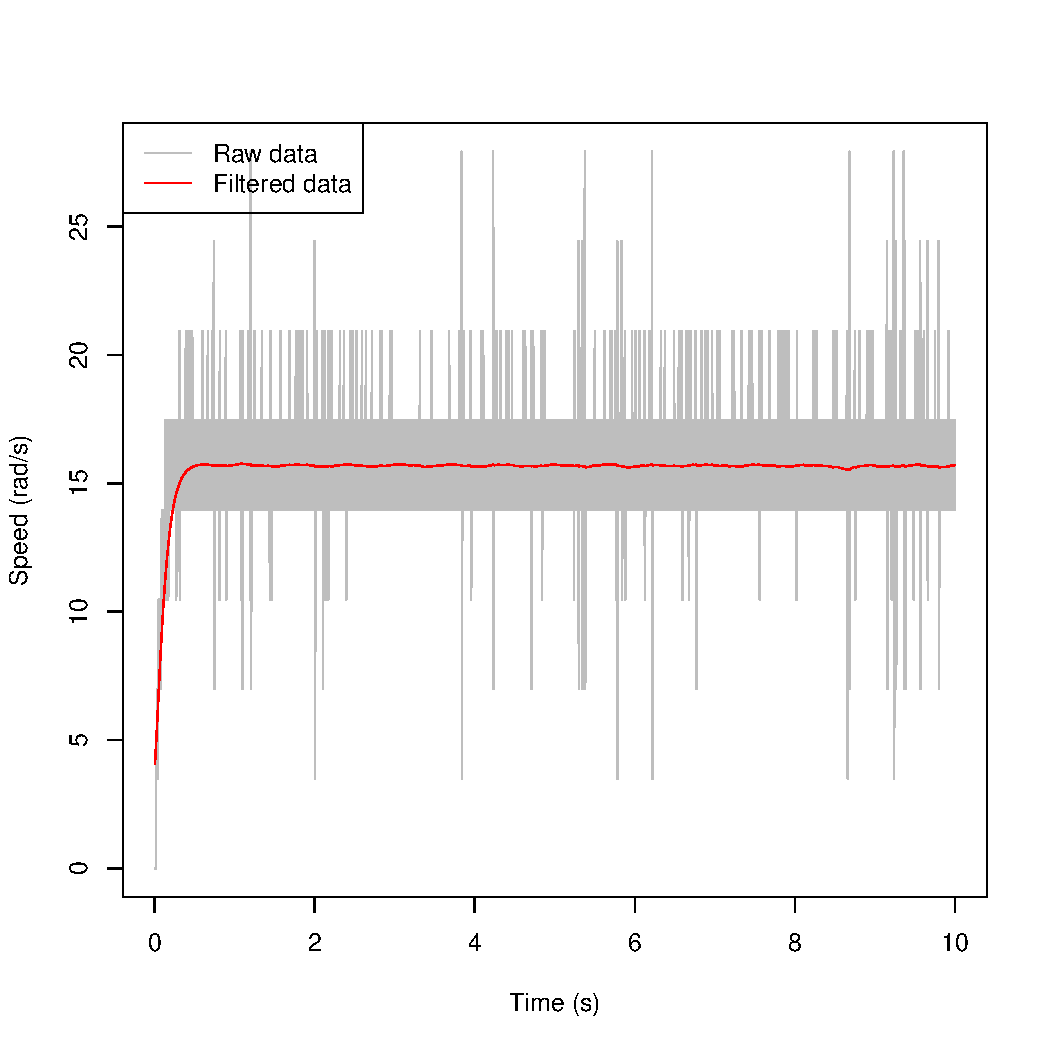
\includegraphics[width=\columnwidth]{../motor_data/plots/filtering/90}
	\caption{Filtered and raw data for motor power = 90.}%
	\label{fig:filtered}%
\end{figure}

\subsection {Parameter Estimation}
We need to estimate 3 parameters $q$, $\omega_{n}$, $\xi$. You can find code in \href{https://github.com/AliaksandrSiarohin/AppliedRobotics/tree/master/identification/identification.r}{Identification}
\subsubsection {Regular method}
For the regular method we use the following formulas:
\begin{equation}
q = \text{Last speed value}
\end{equation}
\begin{equation}
\xi = \sqrt{\frac{\log(\text{overshot}) ^ 2}{\pi ^ 2 + \log(\text{overshot}) ^ 2}}
\end{equation}
\begin{equation}
\omega_{n} =  \frac{\log(\frac{alpha}{100}) -\log(\frac{1}{\sqrt{1-\xi^2}})}{-\text{settling time} * \xi}
\end{equation}
Using this method we obtain 10 sets of parameter which can be seen in \cref{table:reg_es}.
\begin{table}
\centering
\caption{Parameters obtained using regular estimation}
\label{table:reg_es}
\csvreader[tabular=cccc,
    table head=\toprule Power & $q$ & $\xi$ & $\omega_{n}$ \\\midrule,
    table foot=\bottomrule
]%
{../motor_data/regular_estimated_params.csv}{power=\p,q=\q,omega=\o, xi=\x}%
{\p & \q & \o & \x}%
\end{table}


\subsubsection {Regression method}
Let $\hat{s_t}$ be the speed at time $t$, and $T$ - finish time, and ${s_t(q, \xi, \omega_{n})}$ will be the speed from our model. The result parameters will be:
\begin{equation}
(q, \xi, \omega_{n}) = arg\max_{q, \xi, \omega_{n}}{\sum_{t=1}^{T}{(s_t(q, \xi, \omega_{n}) - \hat{s_t}) ^ 2}}
\end{equation}
Using this method we obtain 10 sets of parameter which can be seen in \cref{table:regres_es}.

\begin{table}
\centering
\caption{Parameters obtained using regression estimation}
\label{table:regres_es}
\csvreader[tabular=cccc,
    table head=\toprule Power & $q$ & $\xi$ & $\omega_{n}$ \\\midrule,
    table foot=\bottomrule
]%
{../motor_data/regression_estimated_params.csv}{power=\p,q=\q,omega=\o, xi=\x}%
{\p & \q & \o & \x}%
\end{table}
\subsubsection {Methods Comparison}
For every set of parameters we plot either modeled data and filtered data as example in \cref{fig:fit_dual}, you can find all the plots in \href{https://github.com/AliaksandrSiarohin/AppliedRobotics/tree/master/motor_data/plots/dual_estimation}{Model comparison plots}.
\begin{figure}[t]%
	\centering
	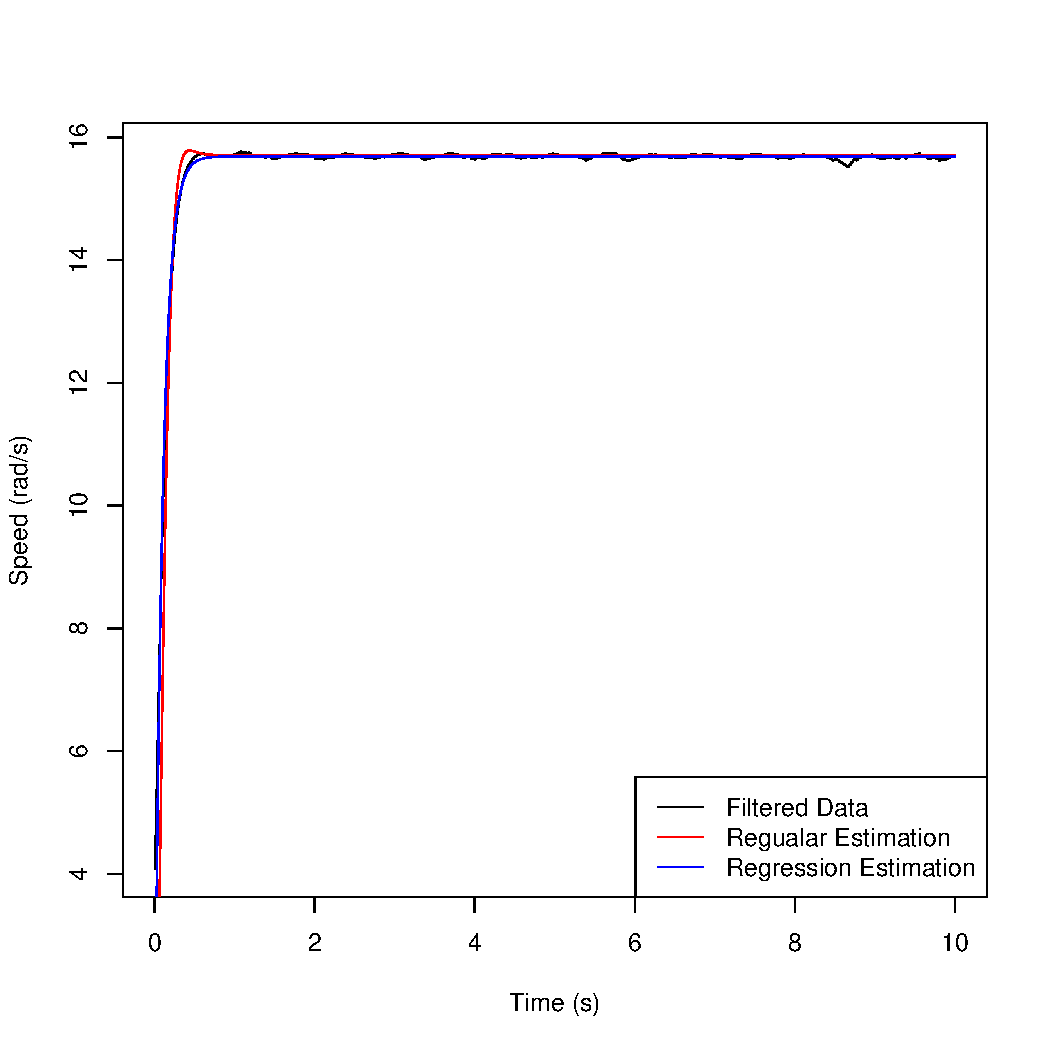
\includegraphics[width=\columnwidth]{../motor_data/plots/dual_estimation/90}
	\caption{Filtered and modeled data for motor power = 90.}%
	\label{fig:fit_dual}%
\end{figure}
For every set of parameters we also compute the mean of mean square errors for all the data sets.
\begin{equation}
\text{result in cell} = \frac{1}{10}\sum_{i=1}^{10}\frac{1}{T}\sum_{t=1}^{T}{(s_t^i(q, \xi, \omega_{n}) - \hat{s_t^i}) ^ 2}
\end{equation}

And we get a result which is in table \cref{table:square_error} (Power is from which data set we obtain a parameters, second column for regular method and third for the regression method). From \cref{table:square_error} we can see that optimal parameters is obtained from (power = 80) data and regression method. We plot filtered data and modeled data with optimal parameters, for example \cref{fig:fit_res}. You can find other plots in \href{https://github.com/AliaksandrSiarohin/AppliedRobotics/tree/master/motor_data/plots/result_estimation}{Result plots}.


\begin{figure}[t]%
	\centering
	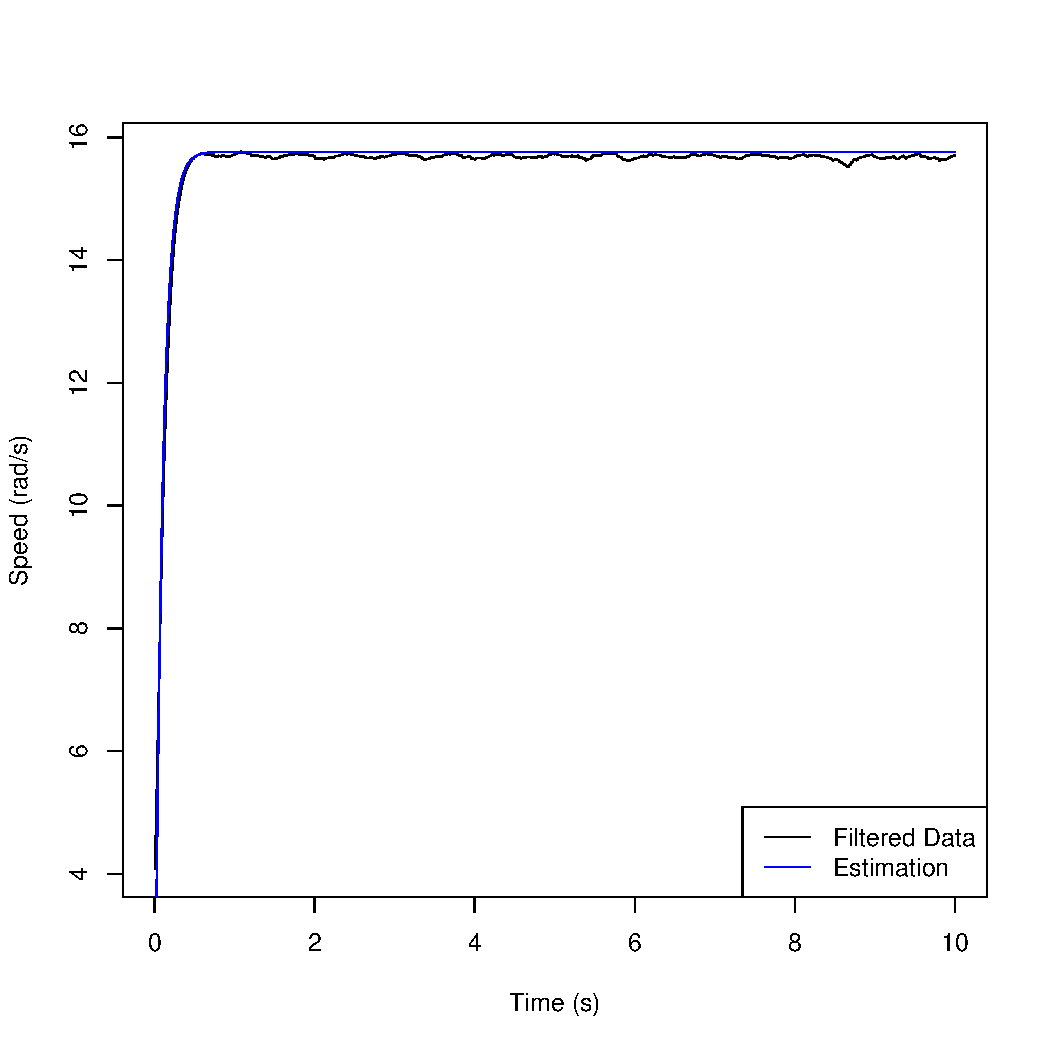
\includegraphics[width=\columnwidth]{../motor_data/plots/result_estimation/90}
	\caption{Filtered and modeled data (with result parameters) for motor power = 90.}%
	\label{fig:fit_res}%
\end{figure}

\begin{table}
\centering
\caption{Mean of mean square error for all data sets.}
\label{table:square_error}
\csvreader[tabular=cccc,
    table head=\toprule Power & Regular Method & Regression Method \\\midrule,
    table foot=\bottomrule
]%
{../motor_data/square_error.csv}{power=\p,regression=\rr,regular=\rg}%
{\p & \rg & \rr}%
\end{table}

\end{document}